%%%%%%%%%%%%%%%%%%%%%%%%%%%%%%%%%%%%%%%%%
% Journal Article
% LaTeX Template
% Version 1.4 (15/5/16)
%
% This template has been downloaded from:
% http://www.LaTeXTemplates.com
%
% Original author:
% Frits Wenneker (http://www.howtotex.com) with extensive modifications by
% Vel (vel@LaTeXTemplates.com)
%
% License:
% CC BY-NC-SA 3.0 (http://creativecommons.org/licenses/by-nc-sa/3.0/)
%
%%%%%%%%%%%%%%%%%%%%%%%%%%%%%%%%%%%%%%%%%

%----------------------------------------------------------------------------------------
%	PACKAGES AND OTHER DOCUMENT CONFIGURATIONS
%----------------------------------------------------------------------------------------
%for images

% /\/\/\/\/\/\/\/\/\/\/\/\/\/\/\/\/\/\/\/\/\/\/\/\/\/\/\/\/\/\/\/\/\/\/\/\/\/\/\
%
% THIS IS IMPORTANT! RUN WITH pdflatex -shell-escape TO AVOID EPS CONVERSION ERROR
%
% /\/\/\/\/\/\/\/\/\/\/\/\/\/\/\/\/\/\/\/\/\/\/\/\/\/\/\/\/\/\/\/\/\/\/\/\/\/\/\

\documentclass[twoside,twocolumn]{article}

\usepackage{graphicx}

\graphicspath{ {../img/} } 

\usepackage{subfig}
\usepackage{todonotes}
\usepackage[sc]{mathpazo} % Use the Palatino font
\usepackage[T1]{fontenc} % Use 8-bit encoding that has 256 glyphs
\linespread{1.05} % Line spacing - Palatino needs more space between lines
\usepackage{microtype} % Slightly tweak font spacing for aesthetics
\usepackage[english]{babel} % Language hyphenation and typographical rules
\usepackage[hmarginratio=1:1,top=32mm,columnsep=20pt]{geometry} % Document margins
\usepackage[labelfont={bf,up},textfont={it,up}]{caption} % Custom captions under/above floats in tables or figures
\usepackage{booktabs} % Horizontal rules in tables

\usepackage{lettrine} % The lettrine is the first enlarged letter at the beginning of the text

\usepackage{enumitem} % Customized lists
\setlist[itemize]{noitemsep} % Make itemize lists more compact

\usepackage{abstract} % Allows abstract customization
\renewcommand{\abstractnamefont}{\normalfont\bfseries} % Set the "Abstract" text to bold
\renewcommand{\abstracttextfont}{\normalfont\small\itshape} % Set the abstract itself to small italic text

\usepackage{titlesec} % Allows customization of titles
\renewcommand\thesection{\Roman{section}} % Roman numerals for the sections
\renewcommand\thesubsection{\roman{subsection}} % roman numerals for subsections
\titleformat{\section}[block]{\large\scshape\centering}{\thesection.}{1em}{} % Change the look of the section titles
\titleformat{\subsection}[block]{\large}{\thesubsection.}{1em}{} % Change the look of the section titles

\usepackage{fancyhdr} % Headers and footers
\pagestyle{fancy} % All pages have headers and footers
\fancyhead{} % Blank out the default header
\fancyfoot{} % Blank out the default footer
\fancyhead[C]{Bird simulation $\bullet$ \today $\bullet$ v1} % Custom header text
\fancyfoot[RO,LE]{\thepage} % Custom footer text

\usepackage{titling} % Customizing the title section
\usepackage{hyperref} % For hyperlinks in the PDF
\usepackage{amssymb,amsmath,bbold,braket}

%----------------------------------------------------------------------------------------
%	TITLE SECTION
%----------------------------------------------------------------------------------------

\setlength{\droptitle}{-4\baselineskip} % Move the title up

\pretitle{\begin{center}\Huge\bfseries} % Article title formatting
\posttitle{\end{center}} % Article title closing formatting
\title{Simulating a flock of birds} %Simulating a flock of birds
\author{%
\textsc{Steffen Randrup, Michel Smola, Andrei Timus}\\[1ex] % Your name
\normalsize University of Copenhagen \\ % Your institution
%\normalsize \href{mailto:john@smith.com}{john@smith.com} % Your email address
%\and % Uncomment if 2 authors are required, duplicate these 4 lines if more
%\textsc{Jane Smith}\thanks{Corresponding author} \\[1ex] % Second author's name
%\normalsize University of Utah \\ % Second author's institution
%\normalsize \href{mailto:jane@smith.com}{jane@smith.com} % Second author's email address
}
\date{\today} % Leave empty to omit a date
\renewcommand{\maketitlehookd}{%
\begin{abstract}
\noindent
In this paper we present a model for studying the behaviour of a group of particles which have some level of interaction between them. The model was inspired from the~\cite{Vicsek} paper\todo[inline]{Present paper and author by name. Also it probably shouldn't be in the abstract} and as in~\cite{Vicsek} the particles have a constant absolute velocity and at each time step  assume the average direction of nearby neighbours with some added perturbation, $\eta$. The behaviour was studied by analysing how the average velocity of the flock $v_a$ varied when parameters like noise, density, number of particles where changed. In addition to $[1]$ we have introduced a cone of vision for every particle and studied the behaviour of the flock in the same conditions. From the simulation results it has been observed that the flock goes through a phase transition where all the particles assume the same direction. The average velocity $v_a$ played the role of an order parameter and it scaled with $(\eta_c-\eta)^\beta$, where $\beta$ is a critical exponent.
\end{abstract}
}

%----------------------------------------------------------------------------------------

\begin{document}
\maketitle

%----------------------------------------------------------------------------------------
%	ARTICLE CONTENTS
%----------------------------------------------------------------------------------------

\section{Introduction}

One may consider the collective movement of birds to be described by a simple set of rules.
In this paper we describe the movement of such a flock as a system of self-propelled particles.
The movement of each bird or particle is governed by the movement of other birds or particles nearby.
In the following we may use birds and particles interchangably.

In our setup the particles where distributed randomly in a square lattice of size L.
Each particle had assigned a random direction $\theta$ and a constant interaction radius r.
One update consisted in modifying the position of all particles according to the following equation:

\begin{equation}
x_{i}(t+1)=x_i(t)+v_i(t)\Delta t
\end{equation}
where $\Delta$t represents the time between 2 updates.
The velocity of a particle had a constant absolute value and a direction given by:
\begin{equation}
\theta(t+1)=\braket{\theta(t)}_r+\Delta \theta
\end{equation} 

where 
\begin{equation}
\braket{\theta(t)}_r=\arctan\frac{\braket{\sin(\theta(t))}_r}{\braket{\cos(\theta(t))}_r}
\end{equation}
is the average direction of the velocities of nearby particles wich are inside the influence circle of radius r of the given particle. $\Delta \theta$ represents the noise in the system and takes values with equal probability within the interval $[-\eta/2,\eta/2]$. For a constant number of particles there are 3 parameters which can be varied: $\eta$,$\rho$,and $v$, where $v$ is the distance a particle travels between 2 updates. $\eta$ describes the interval in which $\Delta\theta$ is picked. $\rho$ is the density of the particles. This is effectively a way of controlling the size of the lattice if the number of particles is fixed.

\begin{figure}[!htb]
	\centering
	\subfloat{{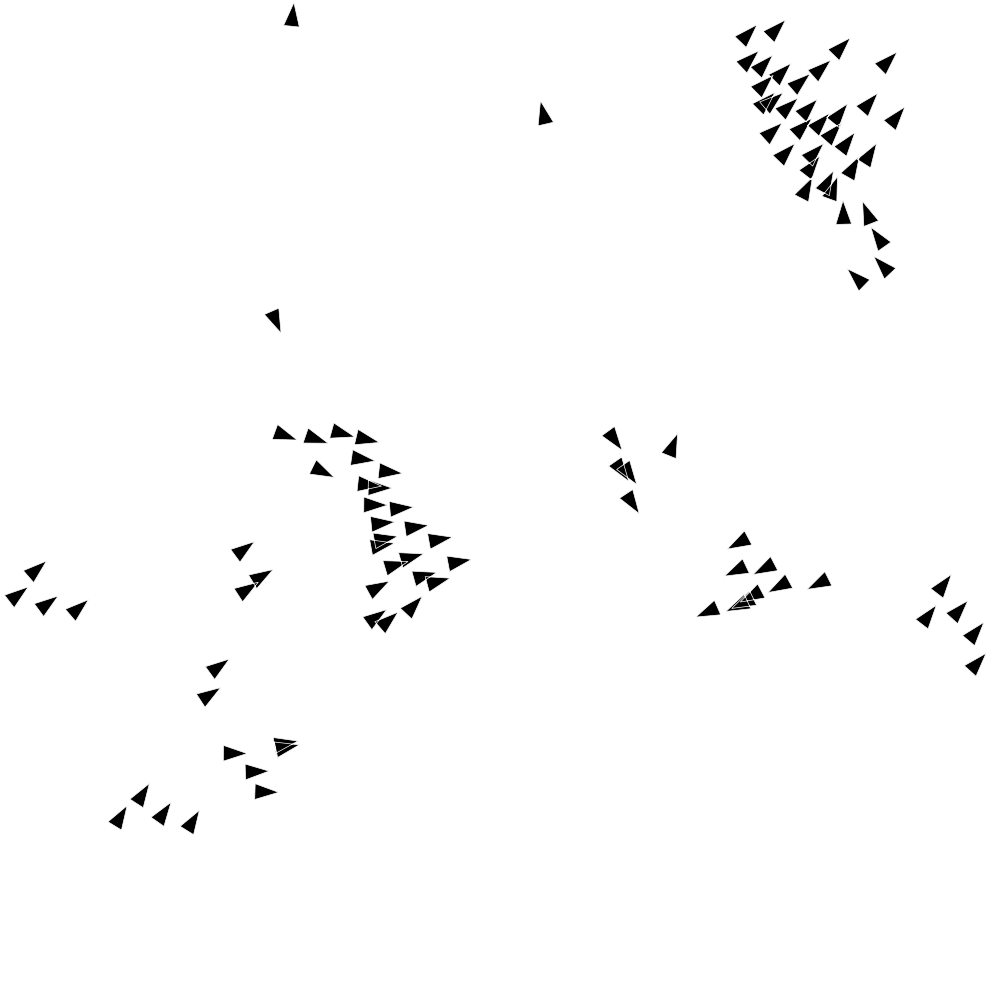
\includegraphics[width=\columnwidth/2]{low-eta-low-rho}}}
  \subfloat{{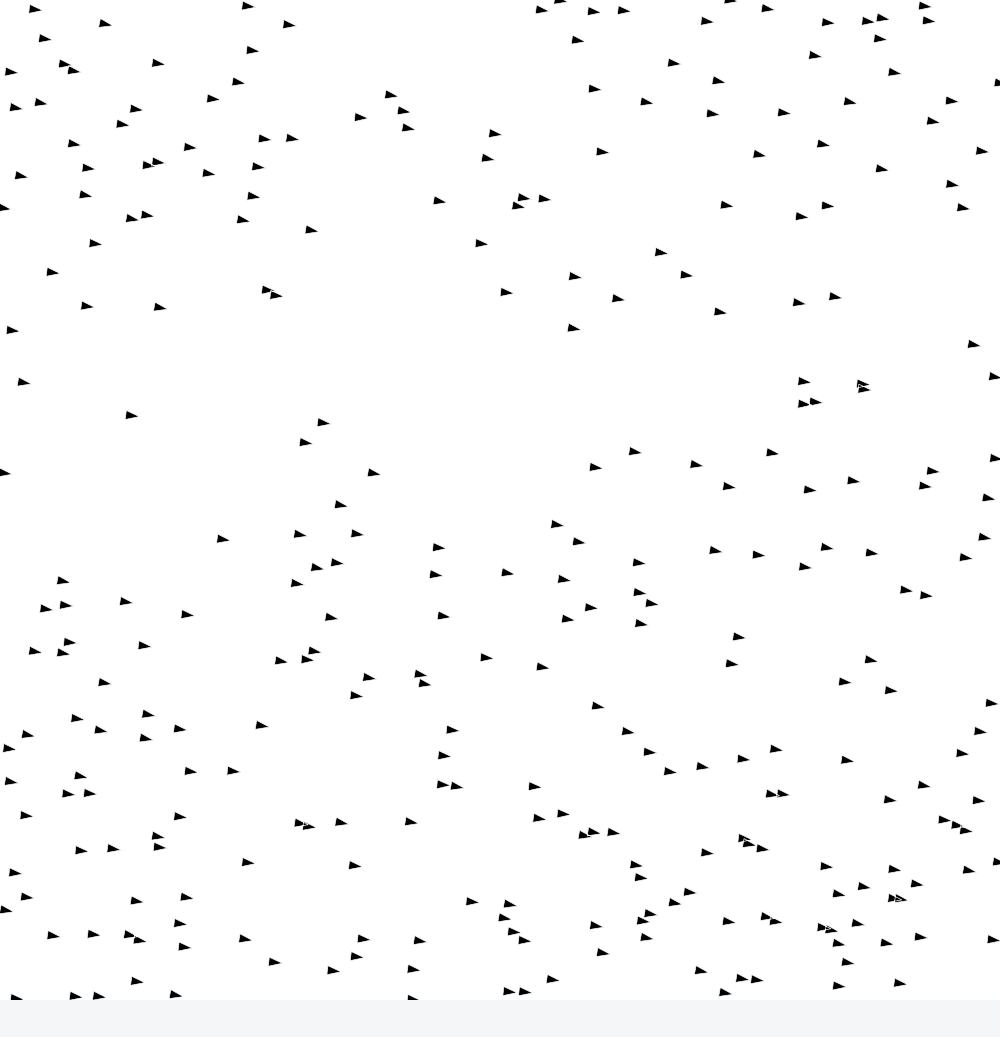
\includegraphics[width=\columnwidth/2]{low-eta-high-rho}}}
	\qquad
	\subfloat{{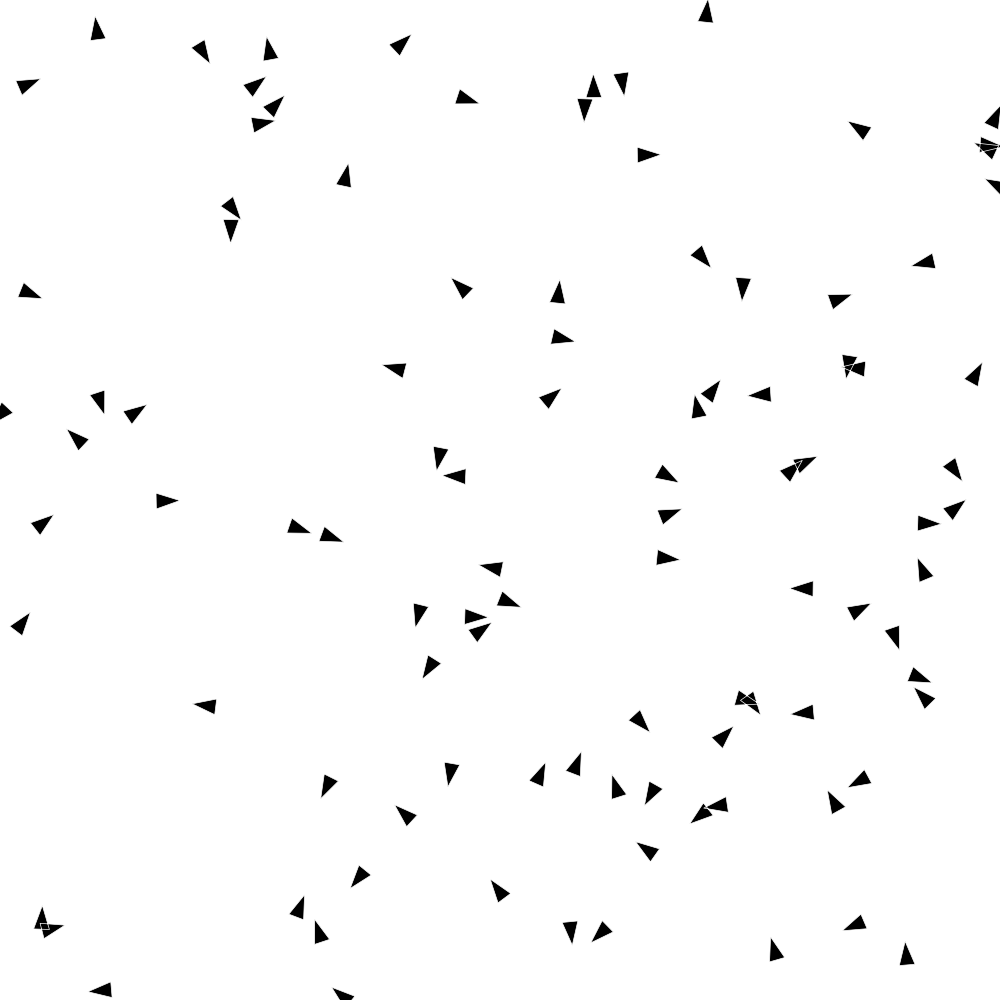
\includegraphics[width=\columnwidth/2]{high-eta-low-rho}}}
	\subfloat{{
\includegraphics[width=\columnwidth/2]{high-eta-high-rho}}}
	\caption{Different configurations of $\eta$ and $\rho$\\Top left: low $\eta$ low $\rho$\\Top right: Low $\eta$, high $\rho$\\Bottm left: High $\eta$, low $\rho$\\Bottom right: High $\eta$, high $\rho$}\label{fig:configs}
\end{figure}

Figure~\ref{fig:configs} shows the configuration of birds for different values of $\rho$ and $\eta$.  
For low values of both $\rho$ and $\eta$ the birds tend to form smaller groups in which the birds move in the same direction.
The groups themselves move randomly.
When the randomness is high and the density low, the overall motion of the birds is just random.
In the case of high randomness and high density, the birds appear to move randomly but with an overall trend in directions
shared among the all the birds.
If the density is high enough, while the noise has low values, the virds move ordly in one direction.
This overall trend in motion is similar to the system going through a kinetic phase transition
where all the particles share the same direction. In order to characterize the behaviour of the flock
we have determined the average normalized velocity of the system and investigated how it changes when the input parameters are modified:

\begin{equation}
v_a=\frac{1}{Nv}\left\vert\sum_{i=1}^{N} v_i\right\vert
\end{equation}

For disordered motion $v_a$ is aproximatively 0, while for ordered $v_a$ has the value near 1.

The behaviour of $v_a$ is found to be similar to that of the order parameter of some equilibrium systems close to their critical point. For large system sizes the data shows scaling which is an indication of a phase transition. Equations~\eqref{eq:va-eta} and~\eqref{eq:va-rho} may be used to describe such a system near the critical value, at which the phase transition occours. 

\subsection{Finding $\eta_c$}
To determine the critical noise parameter $\eta_c$ we used a quadratic fit model
to to fit the falling curve for $\eta < \eta_c$ and a linear fit for $\eta > 
\eta_c$, both visible in figure~\ref{fig:va_over_eta}. $\eta_c$ is then set to 
the intersection of the fit curves. Hereby we determine
\begin{align}
\eta_c = 4.56***
\end{align}
\todo[inline]{put in final number}


\begin{equation}
  \label{eq:va-eta}
  v_a \approx{[\eta_c(\rho)-\eta]}^\beta 
\end{equation}
\begin{equation}
  \label{eq:va-rho}
  v_a \approx{\left[\rho-\rho_c (\eta)\right]}^\gamma
\end{equation}

We further extend the model by implementing a cone-like vision. This means, that 
rather than averaging the velocities over all birds within a certian radius, we 
only look at a slice of this circle. For a bird to be within the vision of 
another bird, it must be within the interaction radius, $r$, and the angle 
between the birds velocities must be within $\pm \theta_{\text{cone}}$. The 
limit $\theta_{\text{cone}} = 2\pi$ equals the case without limiting the
cone vision and reprocuces the results from~\cite{Vicsek}.


\section{Results}

The alignment, $v_a$, depends on the amount of randomness $\eta$ in the system 
and the density $\rho$, as seen in equations~\eqref{eq:va-eta} and~\eqref{eq:va-rho}.
In figure~\ref{fig:va_over_eta} we see how the alignment of 
the birds decreases as the randomness of their motion increases. The decrease 
is to be expected, as a higher degree of randomness should disrupt alignment. 
This reflects to $v_a$, which approaches $0$ in a totally unordered state and $1$
in a totally ordered state.
What might be more interesting is the general shape of the curves. We may then 
determine $\beta$ from equation~\eqref{eq:va-eta} to be \todo[inline]{get value of $\beta$}
This is also shown in figure~\ref{fig:criticaleta}. The results presented here 
are all computed without the conevision (equivalent to $\theta_{\text{cone}} = 2\pi$). 
Figure~\ref{fig:va_over_eta} shows how $v_a$ varies with the noise $\eta$ and 
density $\rho$ for a constant value of density and noise respectively.
As seen in the graph the overall alignment of the particles depends 
on the noise and for a high number of particles N the system becomes less ordered. 
For high $\eta$ the flock reaches a coherent moving phase, while for low $\eta$ 
the particles move randomly in the lattice.  


\begin{figure}[!htb]
  \centering
  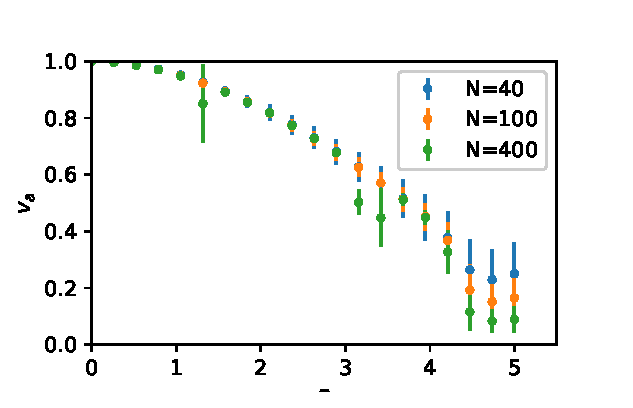
\includegraphics[width=\columnwidth]{va_over_eta}
  \caption{Dependence of alignment on randomness}\label{fig:va_over_eta}
\end{figure}


\begin{figure}[!htb]
	\centering
	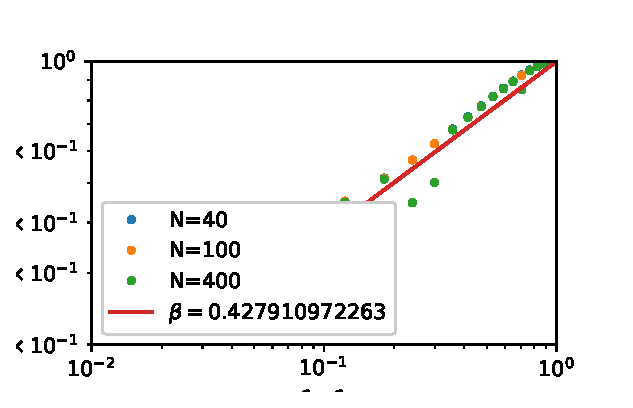
\includegraphics[width=\columnwidth]{va_over_etac_minus_eta_over_etac}
	\caption{Determining $\beta$}\label{fig:criticaleta}
\end{figure}

Similarly we may see the effects of the density on the alignment of birds. This also fits the prediction from equation~\eqref{eq:va-rho}\todo[inline]{Does the effect of density fit the prediction?}. This is shown in figure~\ref{fig:va_over_rho}.

\begin{figure}[!htb]
	\centering
	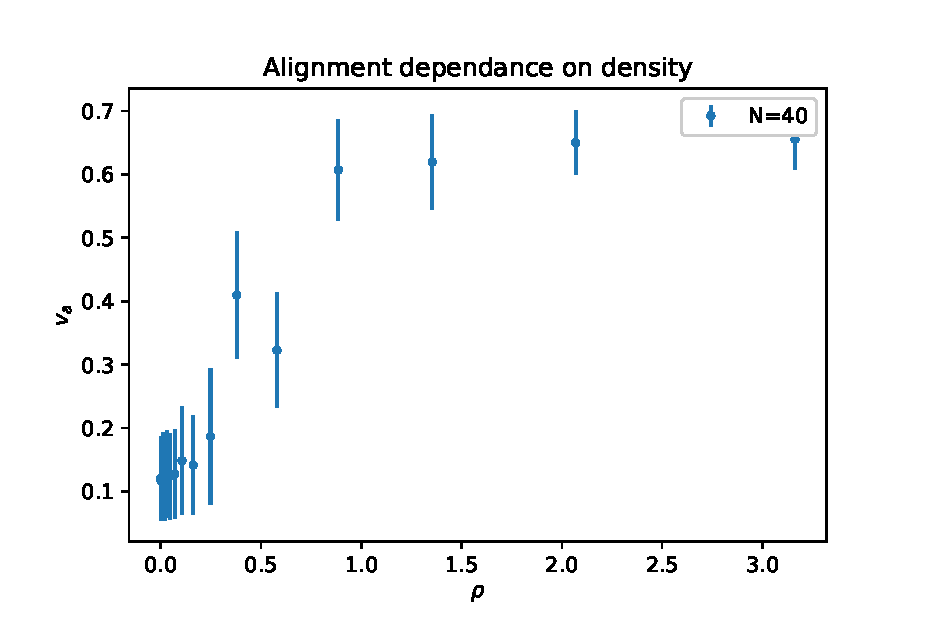
\includegraphics[width=\columnwidth]{va_over_rho}
	\caption{Dependance of alignment on density}\label{fig:va_over_rho}
\end{figure}

\subsection{Cone-like vision}
\label{subsec:conevision}

The effects of our implementation of an angle based vision are only detectable on both low randomness and low density.
This is expected as a higher density causes an effective long range interaction, which may span the entire flock.
This negates the effect of an angle based vision as the flock moves in a coherent fashion.
As for randomness of motion it decreases the overall alignment of the flock as seen in figure~\ref{fig:va_over_eta}.
In figure~\ref{fig:conevision} we present the overall alignment's dependance of the angle describing this cone-like
vision for different densities. The randomness is kept at a low value of $\eta=0.1$.
The results correspond quite well with our expectation of increasing the alignment with larger angle.
For an angle of 180 degrees we see, the alignment looks like it did when we considered every bird within the interaction radius.
We also notice the effects of the density of birds. As described above we expect a long range interaction
between the birds to arise when the density increases.
This effect is visible in the figure as we see the alignment increase faster, when the density is higher.

\begin{figure}[!htb]
\begin{center}
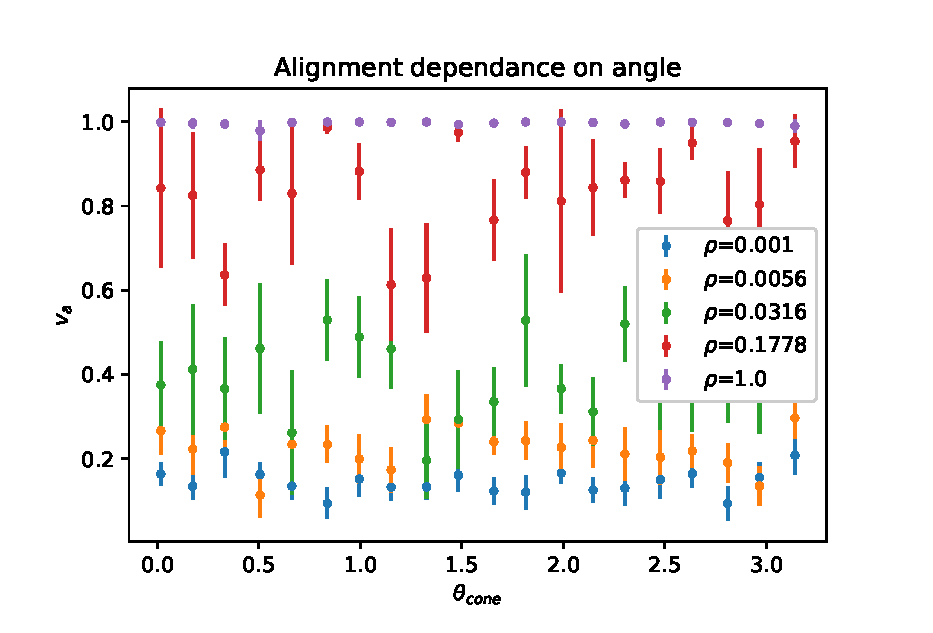
\includegraphics[width=\columnwidth]{va_over_angle}
\end{center}
\caption{Conevision}\label{fig:conevision}
\end{figure}

\section{Discussion}

We have compared the collective motion of birds to a phase transition.
The connection between these is not obvious. However we do see simlilarities in how increasing the noise in the system
will distrupt alignment and how denser systems will display longer effective interaction range. Causing the entire
system to behave coherently.

The addition of a cone-like vision is, as the name might suggests, inspired from birds rather than the study of phase transitions.
The effects of the vision based approach were suttle. They were only detectable for low densities and noise, and for
sufficiently large angles of vision the system would again display behavior to that without the vision based approach.

The values of $v_a$ have been taken as a time average after some transient time after which the system has settled into a state, which doesn't change significantly.

\section{Conclusion}

In this paper we have presetend a model for studying the behaviour of interacting particles. The interaction between particles consisted in maintaining the average velocity of nearby neighbours. The system was studied when particles shared a common interaction radius and when each particle had a cone of vision. During the simulation it has been observed that the system goes through a phase transition where all particles assume the same direction. In order to describe the transition we have calculated the average normalized velocity va and investigated how it behaves when we modify the parameters of the system. In the thermodynamic limit va can be described using (5) or (6).
By plotting these equations we have found  the critical exponent $\beta$ to be equal to\todo[inline]{$\beta$}


%----------------------------------------------------------------------------------------
%	REFERENCE LIST
%----------------------------------------------------------------------------------------

\begin{thebibliography}{99} % Bibliography - this is intentionally simple in this template

  \bibitem{Vicsek}Tamás Vicsek, András Czirók, Eshel Ben-Jacob, Inon Cohen and Ofer Shochet\\
  Novel Type of Phase Transition in a System of Self-Driven Particles\\
  Physical Review Letters, Volume 75, Number 6, August 1995
 
\end{thebibliography}

%----------------------------------------------------------------------------------------

\end{document}
